\chapter{Introducción específica} % Main chapter title

\label{Chapter2}

%----------------------------------------------------------------------------------------
%	SECTION 1
%----------------------------------------------------------------------------------------
Este capítulo da una introducción detallada del sistema SN-17 y el protocolo CAN. También, se presentan algunas características de las entradas y salidas de los controladores industriales PLCs y se explican los distintos componentes seleccionados para el trabajo y su funcionamiento.

\section{Especificaciones SN-17}

El sistema SN-17 se desarrolló para controlar motores \textit{stepper} pequeños que sigan los estándares NEMA (\textit{National Electrical Manufacturers Association})\citep{web_nema}. Estos son estándares ampliamente utilizados para este tipo de motores, que indican las dimensiones que deben tener. 

El sistema SN-17 consiste en una plaqueta electrónica que se monta en la parte trasera del motor. Las dimensiones de estas plaquetas permiten el montaje directo con motores del tipo NEMA-17. En la Figura \ref{fig:dimensiones_nema_17} se presentan las dimensiones de los motores que cumplen con el estándar. Mediante una adaptación mecánica, también se puede emplear la plaqueta para controlar motores de menor o mayor tamaño, siempre y cuando sean del tipo \textit{stepper} y no requieran corrientes mayores a 2 A.

\begin{figure}[htbp]
	\centering
	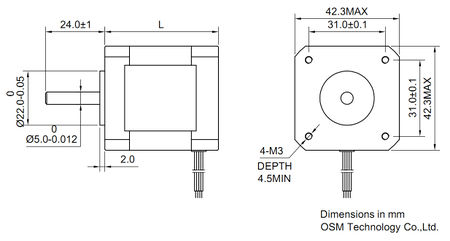
\includegraphics[scale=.9]{./Figures/nema17.jpg}
	\caption{Dimensiones NEMA 17\protect\footnotemark}
	\label{fig:dimensiones_nema_17}
\end{figure}

\footnotetext{\url{https://reprap.org/wiki/NEMA_17_Stepper_motor}} %Link a imagen de dimensiones nema17

Las características electrónicas del sistema SN-17 son:

\begin{itemize}
	\item Alimentación de 12 a 48 V DC: para la operación del motor, de la placa y, opcionalmente, las entradas y salidas industriales.
	\item Regulación de 5 V para electrónica interna.
	\item Microcontrolador ATSAMC21\citep{web_ATSAMC21G18A} con \textit{core ARM Cortex-M0+} y periférico controlador de CAN.
	\item \textit{Driver} de motor del tipo doble puente H\citep{web_A4954}.
	\item \textit{Encoder} magnético absoluto\citep{web_AS5047D} para sensar la posición angular del motor.
	\item \textit{Transceiver} CAN para adaptar las señales de comunicación del bus.
	\item Subcircuito de entradas y salidas discretas PNP optoacopladas\citep{web_optoacopladores_LTV}, con alimentación separada, para interacción con controladores industriales.
\end{itemize}

El sistema funciona mediante un ciclo de control de lazo cerrado del tipo PID\citep{paper_PID_steppers} al cual se le indica un valor deseado (\textit{set point}) de posición, velocidad o torque. Esta información se compara con los valores obtenidos del encoder y se determina como deben ser alimentadas las bobinas del motor para alcanzar el \textit{set point}. Para que el sistema opere correctamente, el \textit{encoder} debe ser calibrado junto con el motor mediante una rutina que genera una tabla de referencia que luego es utilizada en operación.

En una capa superior al control mencionado corre una aplicación en la que se cargan programas que el motor debe realizar. Estos programas estan compuestos de instrucciones configurables que permiten establecer los modos de control deseados (posición, velocidad o torque), los \textit{set points} y errores admisibles para estos (\textit{thresholds}), una limitación del torque para esa instrucción, los tiempos que deben cumplirse para considerar correcta la instrucción (\textit{hold time}) y los tiempos para que se considere que el sistema entró en estado de error (\textit{timeout}). También cuenta con instrucciones para el control del flujo de programa, interacción con las entradas y salidas y comunicaciones a través del puerto CAN.

Existen también configuraciones que se le pueden aplicar al motor. Estas son:
\begin{itemize}
	\item Constantes PID del lazo de control.
	\item Tipo de rutina de \textit{homing} del motor.
	\item Funcionamiento de entradas y salidas.
	\item Guardado de posiciones de eje en memoria.
\end{itemize}

El sistema también puede recibir comandos de forma manual:
\begin{itemize}
	\item Calibración de encoder con motor.
	\item Activación o apagado de motor.
	\item Cerado de motor.
	\item Activación de salidas.
\end{itemize}

En la Tabla \ref{tab:sn17_hoy} se resume la información sobre las distintas funciones que la aplicación del sistema SN-17 puede realizar.

\begin{table}[h]
	\centering
	\caption[Operaciones SN-17]{Funciones de SN-17}
	\begin{tabular}{c c c}    
		\toprule
		\textbf{Señal} 	 & \textbf{Tipo}  & \textbf{Descripción}\\
		\midrule
		Tipo de instrucción & Instrucción 	& Define la instrucción\\		
		Límite de torque 	& Instrucción	& Torque máximo de instrucción \\
		Modo de control		& Instrucción 	& Posición, velocidad, torque \\
		\textit{Set point}	& Instrucción 	& Valor de lazo de control \\
		\textit{Threshold}	& Instrucción 	& Valor de error admisible \\
		\textit{Hold time}	& Instrucción 	& Tiempo de cumplimiento \\
		\textit{Timeout}	& Instrucción 	& Tiempo de no cumplimiento \\
		Guardar posición	& Configuración & Guarda posición actual \\
		Constantes PID		& Configuración & Constantes lazo de control \\	
		Entradas y salidas	& Configuración & Funcionamiento de las IO \\
		\textit{Homing}		& Configuración & Establece rutina de cerado \\	
		Calibración			& Comando		& Inicia la rutina de calibración \\
		Activar motor		& Comando		& Enciende/apaga el motor \\
		\textit{Go Home}	& Comando		& Inicia la rutina de cerado \\
		Activar salidas		& Comando		& Enciende/apaga salidas \\	
		\bottomrule
		\hline
	\end{tabular}
	\label{tab:sn17_hoy}
\end{table}

\section{Características del protocolo CAN}
\label{caracteristicas_can}

Como se trató en el capítulo 1, el protocolo CAN está estandarizado bajo la norma internacional ISO 11898\citep{web_ISO_CAN}. El estándar abarca solamente las capas física y de enlace de datos, es decir las 2 capas más bajas en un modelo OSI (\textit{Open System Interconection}), como el que se presenta en la Figura \ref{fig:modeloOsi}. Para las capas superiores, existen otros estándares, como CANOpen\citep{web_canopen}, del cual se tomaron ideas para este trabajo, pero no se implementa en si.

\begin{figure}[htbp]
	\centering
	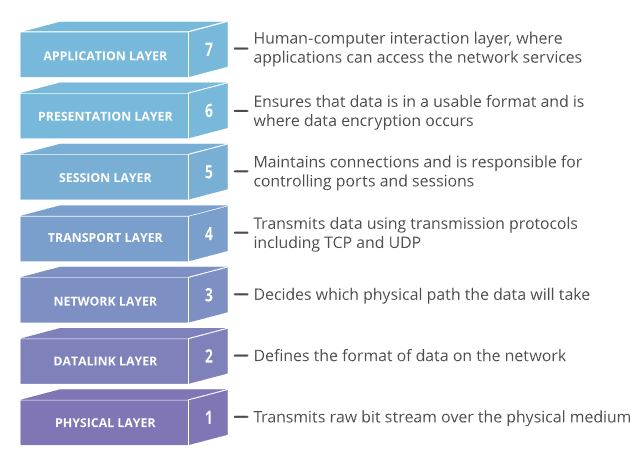
\includegraphics[scale=.8]{./Figures/OSI_model.JPG}
	\caption{Modelo de capas OSI\protect\footnotemark}
	\label{fig:modeloOsi}
\end{figure}

\footnotetext{\url{https://www.cloudflare.com/es-es/learning/ddos/glossary/open-systems-interconnection-model-osi/}} %Link a imagen de modelo OSI

Otras características de la red se relacionan con el armado del circuito de los nodos, el cual suele estar especificado en las hojas de datos de los \textit{transceivers}, así como la necesidad de colocar una resistencia de terminación en los extremos de la red, como puede visualizarse en la Figura \ref{red_can_con_resistores}. El valor de esta resistencia depende de muchas variables, como el largo de la red y la velocidad de transmisión, y se emplean guías para seleccionarlas. Los medios físicos de transmisión, así como los conectores no estás especificados por la norma, aunque existen recomendaciones\citep{Embedded_Networking_CAN}.

\begin{figure}[htbp]
	\centering
	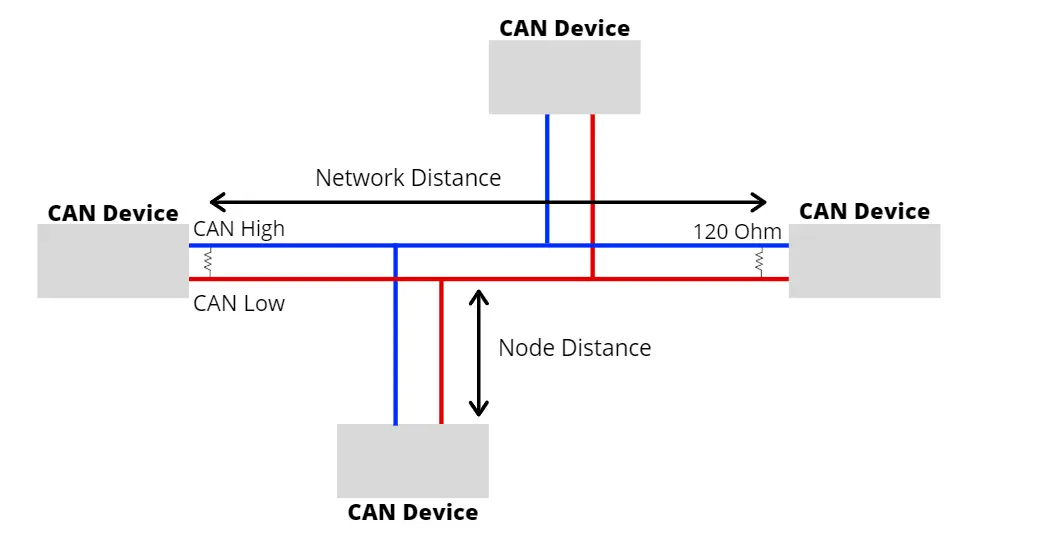
\includegraphics[scale=.6]{./Figures/canBus.png}
	\caption{Esquema de red CAN con resistores de terminación\protect\footnotemark}
	\label{fig:red_can_con_resistores}
\end{figure}

\footnotetext{\url{https://www.seeedstudio.com/blog/2019/11/27/introduction-to-can-bus-and-how-to-use-it-with-arduino/}} %Link a imagen de Red CAN

Las señales usadas son del tipo diferencial y se clasifican en dominantes y recesivas. Una señal dominante en el bus tiene prioridad por sobre una señal recesiva, lo que permite que varios dispositivos estén conectados y puedan hablar al mismo tiempo y que se puedan detectar colisiones\citep{Embedded_Networking_CAN}. En un estado recesivo, las líneas CAN-H y CAN-L están al mismo nivel de tensión. En un estado dominante, CAN-L baja mientras que CAN-H sube generando una diferencia entre ambos. 

El estándar subdivide el tiempo de un bit en distintos segmentos: Sincronización, propagación, fase 1 y fase 2. Estos se describen en una unidad de tiempo menor, referida como \textit{time quanta}. Para un buen funcionamiento de la red, todos estos parámetros deben ser correctamente configurados en los distintos nodos CAN.

En lo que respecta a las tramas CAN, existen de 2 tipos: estándar y extendida. En este trabajo el enfoque está en las tramas estándar que se caracterizan por tener un identificador de 11 bits, donde se codifica información del receptor del mensaje. En la Figura \ref{fig:trama_can} se puede ver un esquema detallando la trama CAN estándar. La trama se separa en:
\begin{itemize}
	\item Comienzo de trama - \textbf{SOF}
	\item Arbitraje
	\item Control
	\item Data a envíar
	\item Verificación
	\item Reconocimiento - \textit{Acknowledge}
	\item Fin de trama - \textbf{EOF}
\end{itemize} 

\begin{figure}[htbp]
	\centering
	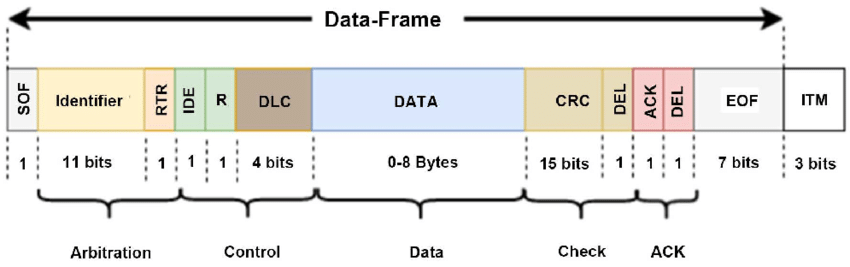
\includegraphics[scale=.4]{./Figures/CANBUS-frame.png}
	\caption{Trama CAN estándar\protect\footnotemark}
	\label{fig:trama_can}
\end{figure}

\footnotetext{\url{https://www.researchgate.net/publication/328607559_Classification_Approach_for_Intrusion_Detection_in_Vehicle_Systems}} %Link a imagen de trama CAN

La sección de arbitraje está compuesta por el identificador y el bit RTR (\textit{Remote Transmission Request}). El identificador es procesado por cada nodo de la red y, mediante el uso conjunto de máscaras y filtros, determinan si el mensaje corresponde a ese nodo o no. También, en caso de que 2 o más nodos quieran transmitir un mensaje al mismo tiempo, el que lo haga con el identificador más bajo será el que tendrá prioridad y tomará el control de la red. Esta funcionalidad se consigue gracias a la lógica AND del circuito del bus. Los nodos que no logran transmitir su mensaje debido a la prioridad inferior pueden reconocer esta situación y retransmitir el mensaje una vez que el bus esté desocupado.

El campo de control del frame tiene al bit IDE, que identifica el tipo de trama entre estándar y extendida, y el DLC, donde se indica la cantidad de bytes que tendrá el mensaje,  pudiendo ser entre 0 a 8.

Luego se encuentran los campos de verificación y reconocimiento. La verificación está compuesta por el campo CRC, que permite comprobar que la información transmitida es igual a la información recibida, es decir, que no hayan ocurrido errores de transmisión. Luego de esto, viene el sector de reconocimiento, donde los receptores reconocen que el mensaje se ha recibido correctamente enviando un bit dominante. La trama termina con una sección de fin de trama.

En la actualidad, se comercializan una gran cantidad de controladores CAN. La gran mayoría ofrece todas las funcionalidades descriptas, que son lo requerido por el estándar. Según la aplicación, se pueden seleccionar controladores que tengan distinto número de filtros y máscaras para identificación de mensajes, tamaño de \textit{buffer} de mensajes, velocidad de operación, entre muchas otras. También, muchos microcontroladores incluyen un periférico de CAN, que suele ser una solución conveniente para implementar redes de este protocolo.

\section{Entradas y salidas de controladores industriales}
\label{io_industriales}

Un PLC (\textit{Programmable Logic Controller}) es un tipo de controlador utilizado para manejar procesos industriales. Se caracteriza por su robustez y su estilo de programación similar a la lógica de relé.

En general, los PLC requieren interactuar con un gran número de sensores y actuadores presentes en un proceso industrial, por lo que cuentan con distintos tipos de módulos de entradas y salidas digitales. Estos módulos adaptan el nível de tensión de las señales que reciben y transmiten, y protegen los circuitos internos del PLC\citep{Introduction_Industrial_Automation}. Normalmente, en el ámbito de la electrónica industrial de control se emplean 24 V de corriente contínua, aunque también es común encontrar 48 V DC o corrientes AC de línea y, en casos poco frecuentes, pueden aparecer otros valores. Los controladores industriales suelen estar preparados para trabajar con la mayoría de estas condiciones.

Uno de los circuitos de acondicionamiento de salidas de PLC se puede observar en la Figura \ref{fig:Circuito_NPN}. En este caso es del tipo NPN, que hace referencia al transistor empleado y al tipo de conexión externa que requiere para su línea común. Es importante notar el uso de un optoacoplador para separar eléctricamente los circuitos y la cantidad de elementos de protección que se agregan para dar robustez.

\begin{figure}[htbp]
	\centering
	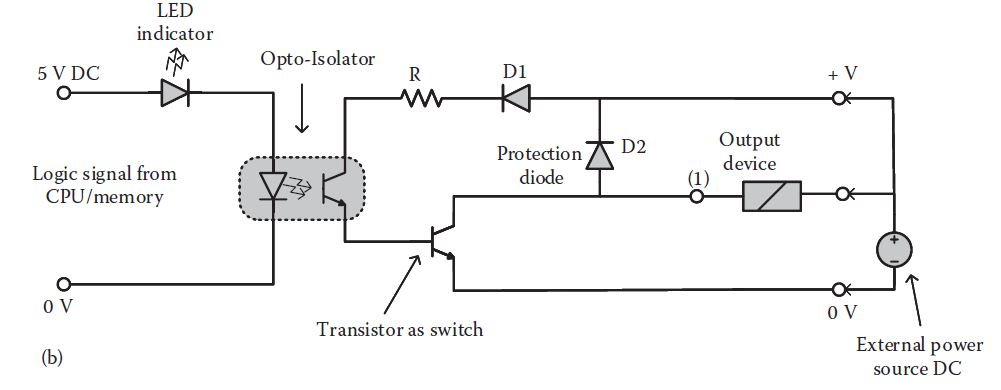
\includegraphics[scale=.5]{./Figures/Circuito_NPN.JPG}
	\caption{Circuito NPN\citep{Introduction_Industrial_Automation}}
	\label{fig:Circuito_NPN}
\end{figure}

Para especificar un módulo de entradas o de salidas se deben determinar los rangos de voltaje y corriente de operación, el consumo máximo de corriente, los valores de tensión lógicos, y la velocidad y frecuencia de conmutación.

\section{Características de componentes electrónicos empleados}

\subsection{Pantallas LCD y conversores I2C}
\label{seccion_display_led}

Las pantallas LCD ofrecen una forma conveniente y económica para generar una interfaz de usuario. Para los proyectos de electrónica, uno de los modelos más populares es el panel de texto basado en el Hitachi HD44780\citep{Arduino_Cookbook}. En la Figura \ref{Pantalla_LCD} se muestra un display de 4 líneas y 20 caracteres por línea. Estos dispositivos solo pueden representar caracteres, no pueden hacer dibujos ni gráficos, por lo tanto las interfaces que se obtienen son sencillas.

\begin{figure}[htbp]
	\centering
	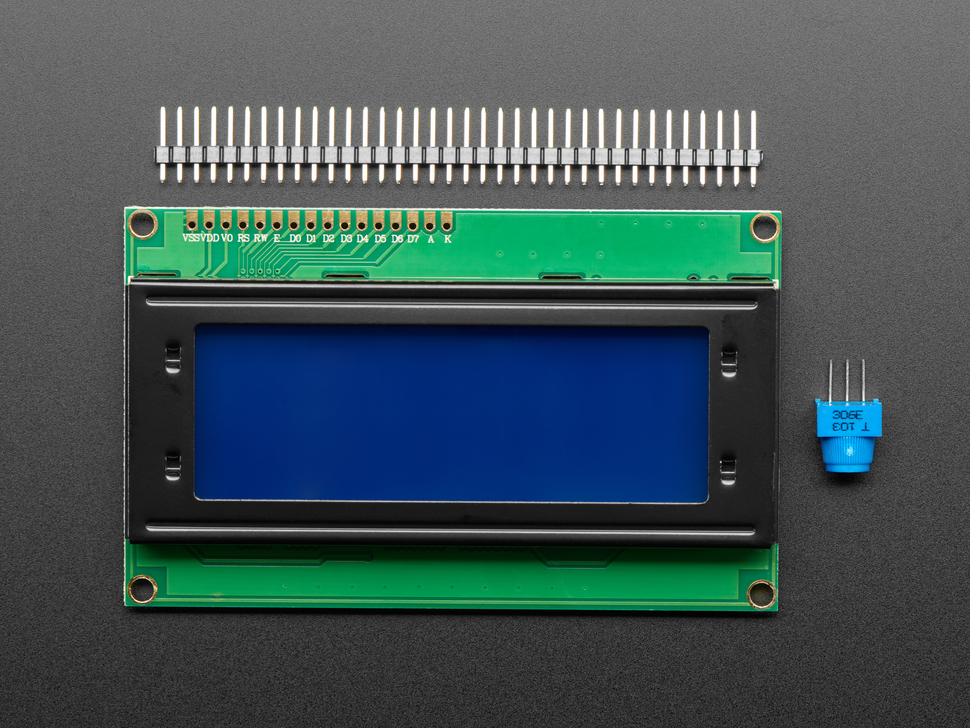
\includegraphics[scale=1.5]{./Figures/LCD.jpg}
	\caption{Pantalla LCD 20x4\protect\footnotemark}
	\label{fig:Pantalla_LCD}
\end{figure}

\footnotetext{\url{https://www.adafruit.com/product/198}} %Link a imagen de LCD

Existen modelos de LCD que incluyen una interfaz I2C (\textit{Inter-Integrated Circuit}), un protocolo de comunicación simple muy utilizado en sistemas embebidos. Esta interfaz facilita la interacción con el display, que normalmente requiere una serie de conexiones discretas para controlarlo. De esta manera, se pueden envíar comandos para modificar la configuración del dispositivo o mostrar texto, según se requiera.

La mayoría de microcontroladores que se emplean en la actualidad poseen un periférico de I2C y sus herramientas de desarrollo proporcionan drivers de este protocolo. I2C se caracteriza por ser del tipo serial y sincrónico. Utiliza 2 líneas de información, SDA y SCL, para transmitir la data y el reloj, respectivamente. En un bus I2C, los distintos dispositivos conectados tienen un código identificador que se emplea para controlar las comunicaciones.

A la hora de implementar una solución con este tipo de pantallas, puede tomarse de referencia alguna de las librerías de código abierto que se encuentran disponibles en la web. Esto puede ayudar a reducir significativamente los tiempos de desarrollo y es el camino que se tomó en este trabajo. En particular, se utilizó la librería \textit{LiquidCrystal\_I2C} para Arduino\citep{web_repo_display_i2c}.

\subsection{Matriz de botones}
\label{teclado}
Las matrices de botones consisten en un conjunto de contactos normalmente abiertos que conectan una fila con una columna cuando se presionan. La metodología de uso consiste en conectar las filas a pines de entrada con resistores de pull-up en el microcontrolador y las columnas a pines de salida. La secuencia que se realiza es poner el nivel de tensión de una columna por vez en bajo (mientras las otras se mantienen en un nivel alto). En ese momento, se leen las entradas de las filas, si alguna está en un nivel bajo es indicación de que el botón de esa fila y columna fue presionado (normalmente estarían en un nivel alto por las resistencias de pull-up)\citep{Arduino_Cookbook}. En la Figura \ref{fig:but_matrix} se puede visualizar un esquema de conexionado de una matriz de botones 4x3 a un microcontrolador. También se muestran los conexionados internos de la matriz, de las filas y las columnas.

\begin{figure}[htbp]
	\centering
	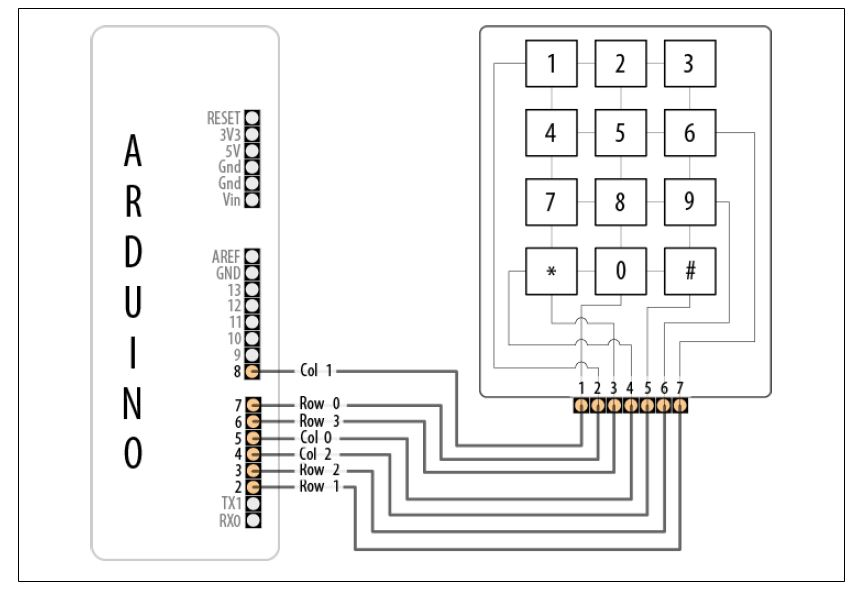
\includegraphics[scale=.6]{./Figures/But_Matrix.JPG}
	\caption{Conexión de matriz de botones 4x3\citep{Arduino_Cookbook}}
	\label{fig:but_matrix}
\end{figure}

Como en el caso de las pantallas LCD, existen muchas librerías de código abierto que implementan soluciones de matrices de botones. Se considera conveniente consultarlas si se desea utilizar uno de estos dispositivos, y es lo que se hizo en este trabajo. En particular, se utilizó la librería Keypad para Arduino\citep{web_repo_keypad}.

\subsection{Conversores UART-USB}
\label{conversor_usb}
El \textit{Universal Asynchronous Receive Transmit} o UART es un protocolo serial de comunicación muy utilizado en sistemas embebidos. Se caracteriza, principalmente, por su sencillez. Como su nombre indica es un protocolo asincrónico (sin línea de clock) que requiere solamente 1 línea para envíar data, o 2 para envíar y recibir.

La mayoría de los microcontroladores que se comercializan en la actualidad disponen de uno o más periféricos de UART. Es común que el propio fabricante provea los \textit{drivers} de implementación para reducir los tiempos de desarrollo.

Otro protocolo ampliamente usado es el USB que suele ser el preferido para interactuar con una PC. Existen en el mercado una gran cantidad de conversores que transforman un mensaje codificado para el protocolo UART a uno USB, permitiendo la interacción entre una PC y un sistema embebido. En general, estos conversores cuentan con \textit{drivers} para los distintos sistemas operativos y son reconocidos por estos, por lo cual solo es necesario conectarlos a través del puerto USB. Desde la PC, cualquier programa de monitoreo de puertos seriales puede usarse para envíar y recibir mensajes con el sistema embebido.

Este tipo de implementaciones suele ser muy útil para realizar operaciones de búsqueda de errores o para armar interfaces gráficas con una PC, facilitando la operatoria de un usuario final. En este trabajo se utiliza uno de estos módulos para esta finalidad.
